% Chapter 1
\mainmatter
\chapter{Software Defined Networking} 

\label{Chapter1} 

Les nouvelles exigences des réseaux modernes en terme d’adaptabilité, d’automatisation, de maintenabilité ont fait naître une nouvelle technologie de réseaux informatique, connue sous le nom de \textit{Software Defined Networking}, qui donne un contrôle centralisé et programmable des ressources réseaux.\\
Ce chapitre donne un aperçu sur l’environnement SDN et montre comment il est conçu  pour répondre aux besoins changeants du réseau.
%----------------------------------------------------------------------------------------

\section{Limites des réseaux traditionnelles}
Avant de passer au Software-Defined Networking, rappelons deux majeures limites des réseaux traditionnels cités par l'ONF (Open Networking Foundation) [\cite{1}] :\\
\begin{itemize}
\item[•] \textbf{Architecture statique et complexe} : pour répondre aux différents niveaux de qualité de service, le volume de trafic élevé et les exigences en matière de sécurité; la technologie réseau est devenue plus complexe et difficile à gérer. Cela a donné lieu à un certain nombre de protocoles définis de façon indépendante dont chacun répond à une partie des besoins de réseautage. Un exemple de la difficulté que cela présente est lorsque les appareils sont ajoutés ou déplacés. Le personnel de gestion du réseau doit utiliser des outils de gestion au niveau de l’appareil pour modifications des paramètres de configuration dans plusieurs commutateurs, routeurs, pare-feu,...etc. Les opérations de mise à jour sont fastidieuses et coûteuses en matière de temps et donnent place aux erreurs de configuration qui peuvent engendrer des problèmes au niveau du réseau.\\
\item[•] \textbf{Scalabilité limitée} : la demande sur les réseaux augmente rapidement, tant en volume qu’en variétés. Ajouter plus de commutateurs ou augmenter la capacité de transmission est difficile en raison de la complexité et nature statique du réseau.
\end{itemize}

%----------------------------------------------------------------------------------------
\newpage
\section{Une approche réseau moderne}
Une approche réseau moderne doit satisfaire les exigences citées par L’Open Data Center Alliance (ODCA)  [\cite{2}], notamment :\\
\begin{itemize}
\item[•] \textbf{Adaptabilité}: les réseaux doivent s’adapter dynamiquement, en fonction des besoins des applications, des activités, la politique et les conditions du réseau.\\
\item[•] \textbf{Automatisation}: les changements de politique doivent être propagé automatiquement afin de réduire le travail manuel et les erreurs.\\
\item[•] \textbf{Sécurité intégrée}: les applications réseau doivent intégrer la sécurité comme service de base et non pas comme solution complémentaire.\\
\item[•] \textbf{Mise à l’échelle sur demande}: les implémentations doivent avoir la capacité à prendre de l’expansion ou à réduire le réseau et ses services pour répondre aux requêtes à la demande.
\end{itemize}

%----------------------------------------------------------------------------------------

\section{Définition}

Software-defined networking est une nouvelle architecture réseau, qui a pour but pratique de rendre programmables les réseaux par le biais d’un contrôleur centralisé. Rappelons que dans les réseaux traditionnels les périphériques réseaux (commutateurs et routeurs) construisent leurs tables de routage localement, ce qui signifie qu’ils prennent leurs propres décisions en interne sur la meilleure façon d’aiguiller le trafic. \\

Dans les SDN les décisions de routage sont prises par un contrôleur centralisé ce qui fait que les périphériques n’ont plus intérêt à prendre des décisions localement, ils n’ont qu’à suivre celles prises par le contrôleur. Ce qui rend cette architecture dynamique, programmable et idéale pour les réseaux modernes à haute demande.

%----------------------------------------------------------------------------------------

\section{Architecture SDN}

Le concept central derrière l’architecture SDN est de permettre aux développeurs et gestionnaires de réseau d’avoir un contrôle centralisé sur les équipements réseau.\\

Le SDN fait la séparation entre le plan de contrôle et le plan de données. Le plan de contrôle est responsable des décisions de transmission, il comprend des mécanismes de transmission d’itinéraire du trafic. Le plan de données représente la partie des commutateurs et routeurs qui assurent effectivement la transmission des données. La différence entre l’architecture traditionnelle  et l’architecture SDN est illustrée dans la figure suivante:

\newpage
\begin{figure}[h]
\centering
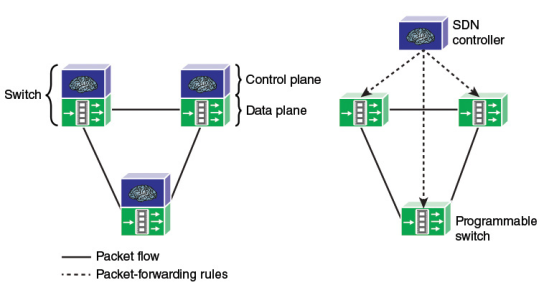
\includegraphics[width=0.7\textwidth]{Figures/SDN_Architecture}
\decoRule
\caption{Plan de données et plan de contrôle}
\label{fig:SDN_Architecture}
\end{figure}

Dans l’architecture traditionnelle le plan de données et le plan de contrôle sont intégrés dans un même équipement physique. Par contre dans Le SDN le plan de contrôle est externalisé de tous les périphériques réseaux et associé à un équipement dit contrôleur.

\begin{figure}[h]
\centering
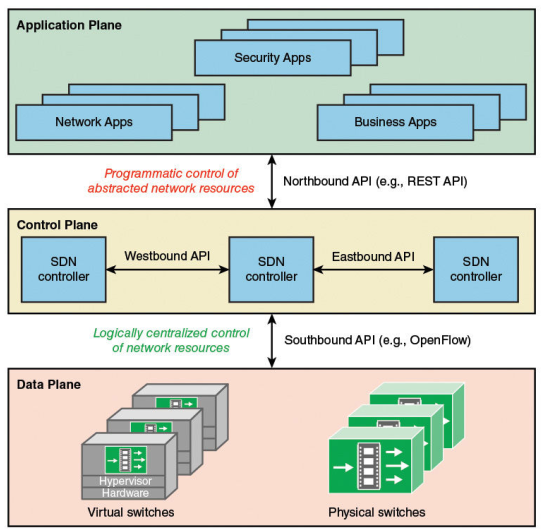
\includegraphics[width=0.55\textwidth]{Figures/SDN_Plans}
\decoRule
\caption{Architecture SDN}
\label{fig:SDN_Plans}
\end{figure}

L’architecture SDN définit trois couches,  comme indiqué dans la figure \ref{fig:SDN_Plans}, chacune représente un plan, plan de données, plan de contrôle ou plan d’application. Chaque couche ne peut communiquer qu’avec ces couches voisines. 

\subsection{Plan de Données}
Le plan de données se compose de commutateurs physiques et de commutateurs virtuels, qui sont responsables de la transmission des paquets. Cependant chaque commutateur doit implémenter un modèle de transfert de paquet, ce modèle est défini à travers une API (Application programming interface) qui réside entre le plan de contrôle et le plan de données permettant la communication entre le contrôleur et les commutateurs du plan de données. Parmi ces API, le OpenFlow, qui nous allons détailler par la suite.\\

\noindent Le plan de données assure une fonction autre que la transmission des données, le support de contrôle. Cette fonction permet la communication avec le contrôleur SDN pour l’échange des informations liées à la gestion du périphérique.  
%----------------------------------------------------------------------------------------

\subsection{Plan de Contrôle}
Le plan de contrôle SDN, composé d’un ou plusieurs contrôleurs, mappe les demandes de service de couche d’application en commandes et directives spécifiques aux commutateurs du plan de données et fournit aux applications des informations sur la topologie et l’activité du plan de données.\\

\noindent Le contrôleur définit les flux de données qui se produisent dans le plan de données. Un flux est une séquence de paquets qui partagent un ensemble de valeurs de champ d'en-tête. Pour qu’un flux traverse le réseau, le contrôleur intervient pour vérifier si ce flux est autorisé dans le cadre de la politique réseau définie.\\

\noindent Dans ce qui suit, trois frameworks les plus utilisés pour la mise en œuvre des contrôleurs SDN:\\
\begin{itemize}
\item[]\textbf{OpenDaylight}[\cite{3}]: Un framework open source, écrit en java, permettant la programmation réseau. OpenDaylight a été développé par Cisco et IBM, il permet à plusieurs contrôleurs distribués, résidants dans des serveurs différents, de fonctionner comme étant un seul contrôleur centralisé.\\
\item[]\textbf{Ryu}[\cite{4}]: Framework open source développé par NTT labs, basé composant et entièrement écrit en python. Ryu fournit des composants logiciels avec API bien définie qui rend la tâche facile aux développeurs pour créer de nouvelles applications de gestion et de contrôle.\\
\item[]\textbf{NOX}[\cite{5}]: Développé par Nicira networks, NOX est une plateforme conçue spécialement pour le développement des applications de contrôle de réseau.
\end{itemize} 

\newpage
\subsection{Plan d'Applications}
Le plan d’application contient des applications et des services qui définissent, surveillent et contrôlent les ressources et le comportement du réseau. Ces applications interagissent avec le plan de contrôle via des interfaces dédiées pour que la couche de contrôle personnalise automatiquement le comportement et les propriétés des ressources réseau. La programmation d’une application SDN utilise la vue abstraite des ressources réseau fournie par la couche de contrôle au moyen d’informations et de modèles de données exposés via l’API fournie.
%----------------------------------------------------------------------------------------

\section{Caractéristiques des SDN}
Après avoir vu la nouvelle architecture réseau, le software-defined Networking, en opposition avec l'architecture traditionnelle,nous trouvons que les principales caractéristiques des SDN sont les suivantes :\\
\begin{itemize}
\item[-]\textbf{Séparation des plans}: le plan de contrôle est séparé du plan de données. Les périphériques de plan de données deviennent des simples dispositifs de transfert de paquets. Le plan de contrôle est installé dans un contrôleur ou ensemble de contrôleurs centralisés et coordonnés.\\
\item[-]\textbf{Programmabilité}: le réseau est programmable par des applications qui s’exécutent au-dessus du contrôleur SDN. Les contrôleurs présentent une vue abstraite des ressources du réseau aux applications.\\
\item[-]\textbf{Centralisation}: le cerveau du réseau est (logiquement) centralisée dans des contrôleurs SDN basé sur des logiciels qui maintiennent une vue globale du réseau.
\end{itemize}

%----------------------------------------------------------------------------------------
\section{OpenFlow et SDN}
\label{S_OpenFlow}
Pour implémenter le concept SDN en pratique, un protocole standardisé et sécurisé est essentiel  pour établir la connexion entre le contrôleur et les ressources réseau. L’architecture Openflow se compose de trois éléments principaux: un commutateur Openflow, un contrôleur externe et le protocole Openflow. Le plan de données et le plan de contrôle communiquent sur un canal sécurisé via ce protocole. Le commutateur Openflow dispose de tables de flux et d’une couche d’abstraction qui communique en toute sécurité avec un contrôleur via le protocole Openflow. La table de flux contient des entrées de flux qui déterminent comment les paquets appartenant à un flux seront traités et transmis. 
Les entrées de flux consistent en :\\

\begin{itemize}
\item[•] Matching rules – pour apparier les paquets entrants.
\item[•] Counters – pour collecter des statistiques du flux.
\item[•] Set of instructions / actions - à appliquer en cas de correspondance.\\
\end{itemize}

Lorsqu’un paquet arrive à un commutateur Open Flow, les champs d’en-tête du paquet sont extraits et comparés aux règles correspondances. Si une correspondance est trouvée, le commutateur applique l’action appropriée. S’il n’y a pas de correspondance, l’action effectuée par le commutateur dépend de l’instruction définie par l’entrée de \textit{ table-miss flow}. Chaque table de flux doit avoir cette entrée afin de gérer la non-correspondance d’un flux dans une table. Des exemples d’actions qui peuvent être effectuées lorsque'aucune correspondance n’est trouvée sont: abandonner le paquet, continuer le processus de correspondance sur la table de flux suivant, acheminer le paquet au contrôleur. 

\subsection{Table de Flux}
La table de flux contient plusieurs entrées. Chaque entrée de cette table a la structure suivante:\\
\begin{table}[h]
\begin{center}
\begin{tabular}{ | c | c | c | c | c | c |}
\hline
\rowcolor[rgb]{0.85,0.85,0.85}
Match Fields & Priority & Counters & Instructions & Timeouts & Cookie\\
\hline
\end{tabular}
\caption{Entrée d'une table de flux}
\end{center}
\end{table}
\begin{itemize}

\item[-]\textbf{Match Fields}: permet de sélectionner des paquets qui correspondent aux valeurs des champs de Match Fields.
\item[-]\textbf{Priority}: un champ sur 16 bits, définit la priorité de l'entrée. la valeur O correspond à la priorité la plus basse.
\item[-]\textbf{Counters}: un conteur de paquets. Il est mis à jour lors d'une correspondance d'un paquet à une entrée de la table de flux. 
\item[-]\textbf{Instructions}: ensemble d'instructions à déclencher en cas de correspondance. 
\item[-]\textbf{Timeouts}: durée de vie d'une entrée de table.
\item[-]\textbf{Cookie}: utilisé par le contrôleur pour le filtrage de paquets.\\
\end{itemize}

Le champ principal dans une entrée de table de flux est le \textbf{Match Fields}, ce dernier définit un vecteur d'attributs correspondant aux champs de l’entête du paquet arrivé au commutateur.\\

\begin{table}[h]
\begin{center}
\begin{tabular}{ | m{0.7cm} | m{0.7cm} | m{0.7cm} | m{0.7cm} | m{0.7cm} | m{0.7cm} | m{0.7cm} | m{0.7cm} | m{0.7cm} | m{0.7cm} | m{0.7cm} | m{0.7cm} | m{0.7cm} | m{0.7cm} |}
\hline
\rowcolor[rgb]{0.80,0.80,0.80}
 Port Ent & Port Srt & Ethr AS & Ethr AD & Ethr Type & IP & AS IPv4 & AD IPv4 & AS IPv6 & AD IPv6 & TCP Src & TCP Dest & UDP Src & UDP Dest\\
\hline
\end{tabular}
\caption{Match Fields}
\end{center}
\end{table}

\begin{itemize}
\item[\textbf{Port Ent}]: Identificateur du port par lequel le paquet est arrivé.
\item[\textbf{Port Srt}]: Identificateur du port de sortie.
\item[\textbf{Ethr AS et Ethr AD}]: Adresses Ethernet, source et destination. 
\item[\textbf{Ethr Type}]: Type de trame Ethernet.
\item[\textbf{IP Type}]: version IP, 4 ou 6
\item[\textbf{AS IPv4 et AD IPv4}]: Adresses IPv4, source et destination.
\item[\textbf{AS IPv6 et AD IPv6}]: Adresses TPv6, source et destination.
\item[\textbf{TCP Src et TCP Dest, UDP Src et UDP Dest}]: Ports source et destination de couche de transport.
\end{itemize}

%----------------------------------------------------------------------------------------
\newpage
\section{Contrôleur SDN}
Comme mentionné précédemment, le contrôleur est le composant principal de toute l'infrastructure SDN où tous les calculs y sont effectués. Il est responsable de la gestion de tout le réseau.\\
En résumé, les fonctions assurées par un contrôleur SDN sont [\cite{6}]: \\

\noindent\textbf{- Routage plus court chemin}: utilise les informations de routage collectées à partir des commutateurs pour établir la table de routage.\\
\textbf{- Gestion de notifications}: reçoit, traite et transmet à un événement d’application, les notifications d’alarme, les alarmes de sécurité et les changements d’état.\\
\textbf{- Sécurité}: fournit des services de sécurité.\\
\textbf{- Gestion de topologie}: construit et maintient les informations sur l'interconnexion des équipements réseau.\\
\textbf{- Gestion de statistique}: collecte et stock des informations sur le trafic réseau.\\
\textbf{- Gestion de périphériques}: configure les paramètres des commutateurs et gère les tables de flux \autoref{S_OpenFlow}.
 

\section{Avantages et inconvénients des SDN}
\subsection{Avantages}
\noindent - Économies opérationnelles: les SDN réduisent les dépenses d’exploitation. Les services de réseau peuvent être gérés par des applications, libérant ainsi l’équipe de réseautage.\\

\noindent - Une meilleure gestion: les SDN offrent une gestion centralisée et automatisée des équipements réseau.\\

\noindent - Flexibilité: les SDN créent une flexibilité dans la façon dont le réseau peut être exploité. Les administrateurs réseau peuvent écrire leurs propres services de réseau en utilisant les outils de développement standard.\\

\noindent - Disponibilité améliorée: en éliminant l’intervention manuelle, les SDN permettent de réduire les erreurs de configuration et de déploiement qui peuvent affecter le réseau. 

\subsection{Inconvénients}
\noindent - Il faut modifier entièrement l’infrastructure réseau  pour mettre en œuvre le SDN. Il faut donc reconfigurer complètement le réseau. Cela implique des dépenses considérables en vue de mettre en œuvre cette technologie.\\

\noindent- SDN à ses propres vulnérabilités de sécurité. Ceci nécessite de mettre en place de nouvelles approches pour veiller sur la sécurité du réseau.\\

\noindent- Toute l'intelligence du réseau est placée dans le contrôleur, ce qui constitue un point de défaillance unique. Si le contrôleur tombe en panne ou il est compromis tout le réseau cessera de fonctionner.

\section{Conclusion}
Le Software Defined Networking annonce des changements importants sur les réseaux dans les années à venir. Ce chapitre n'a parlé que brièvement sur cette nouvelle technologie, sa définition est bien plus vague et son domaine d'application est bien plus large. Les profits qui peuvent être tirés de cette technologie sont innombrables si bien exploitée.
